\ifdefined\included
\else
\documentclass[french, a4paper, 11pt, twoside, pdftex]{StyleThese}
\usepackage{iflang}
\usepackage{bibentry}



%\usepackage[sectionbib]{chapterbib}          % Cross-reference package (Natural BiB)
%\usepackage{natbib}                  % Put References at the end of each chapter
%\usepackage{bibunits}
% Do not put 'sectionbib' option here.
% Sectionbib option in 'natbib' will do.


\usepackage{fancyhdr}                    % Fancy Header and Footer

\usepackage[utf8]{inputenc}
\usepackage[T1]{fontenc}
\usepackage[french]{babel} %
\usepackage{lmodern} \normalfont %to load T1lmr.fd 
\DeclareFontShape{T1}{cmr}{b}{sc} { <-> ssub * cmr/bx/sc }{}
%\hyphenation{gar}

\usepackage{amsmath,amssymb}             % AMS Math
\usepackage{nicefrac}
\usepackage{siunitx}					%% Unites Math SI

\usepackage{blindtext}

\usepackage{datetime}

\usepackage{lipsum} 

\usepackage[inline]{enumitem}

\usepackage{hhline}
%\usepackage[left=1.5in,right=1.3in,top=1.1in,bottom=1.1in]{geometry}
\usepackage[left=1.5in,right=1.3in,top=1.1in,bottom=1.1in,includefoot,includehead,headheight=13.6pt]{geometry}

%%\renewcommand{\baselinestretch}{1.05}

%%%%%%%% Multi-figures avec sub-captions
\usepackage{caption}
\usepackage{subcaption}

% Table of contents for each chapter

\usepackage[nottoc, notlof, notlot]{tocbibind}
\usepackage[nohints]{minitoc}
\setcounter{minitocdepth}{2}
\mtcindent=15pt
% Use \minitoc where to put a table of contents

\usepackage{aecompl}

%% Package cosmetic meilleur layout du texte en jouant sur le spacing par caractères
\usepackage[activate={true,nocompatibility},final,tracking=true,kerning=true,factor=1100,stretch=10,shrink=10]{microtype}
\usepackage[absolute,overlay]{textpos} 
\setlength{\TPHorizModule}{\paperwidth}\setlength{\TPVertModule}{\paperheight}
\sloppy

%%%%%%%%%%% JOLIS TABLEAUX
\usepackage{tabularx}		%\usepackage{tabular}
\usepackage{longtable}
\usepackage{multirow}
\newcommand{\mc}{\multicolumn} 
\newcommand{\mr}[2]{\multirow{#1}{*}{#2}} 	\newcommand{\mrQ}{\multirow{-4}{*}}
\usepackage{booktabs}

\usepackage[usenames,dvipsnames]{xcolor} 

\makeatletter
\newcommand{\ccolor}[3][]{%
	\kern-\fboxsep
	\if\relax\detokenize{#1}\relax
	\expandafter\@firstoftwo
	\else
	\expandafter\@secondoftwo
	\fi
	{\colorbox{#2}}%
	{\colorbox[#1]{#2}}%
	{#3}\kern-\fboxsep
}
\makeatother

%%%%% Insertion graphiques format PGF
\usepackage{pgfplots}
\pgfplotsset{width=\linewidth, compat=1.16}%, compat=1.17}
\usepackage{adjustbox}          %%% PERMET DE LES RECADRER + FACILEMENT


%%%%%%%%%% Bullets de listes sans saut de ligne %%%%%%%%%%
\usepackage{xparse}

\ExplSyntaxOn%
\seq_new:N \l_local_enum_seq

\newcommand{\storethestuff}[1]{%
  \seq_set_from_clist:Nn \l_local_enum_seq {#1}%
}

\newcommand{\dotheenumstuff}{%
\int_zero:N \l_tmpa_int
\seq_map_inline:Nn \l_local_enum_seq {%
    \int_incr:N \l_tmpa_int% Increase the counter
    \item ##1
    % Check whether the list has reached the end -- if so, use '.' instead of ','
    %\int_compare:nNnTF 
    % { \l_tmpa_int } < {\seq_count:N \l_local_enum_seq} 
    % {,} {.}
  }
}
\ExplSyntaxOff

\NewDocumentCommand{\linebullets}{+m}{%
  \storethestuff{#1}%
  \begin{enumerate*}[label={\alph*)},font={\bfseries},itemjoin={{, }}]
    \dotheenumstuff%
  \end{enumerate*}
}

\newcommand{\cmnt}[1]{}  %%%%% AJOUT DE COMMENTAIRE MULTILIGNES


%%%%%%%%%% ECRITURE CARACTERES DANS UN CERCLE %%%%%%%%%%
%\def\circleTxt[#1]{\raisebox{.5pt}{\textcircled{\raisebox{-1pt}{#1}}}}
\newcommand{\ctxt}[1]{\raisebox{.5pt}{\textcircled{\raisebox{-1.2pt}{#1}}}}
% Glossary / list of abbreviations

\usepackage[intoc]{nomencl}
\IfLanguageName{english}{%
\renewcommand{\nomname}{Glossary}
}{ %
\renewcommand{\nomname}{Liste des Abréviations}
}

\makenomenclature

% My pdf code

\usepackage{ifpdf}

\ifpdf
  \usepackage[pdftex]{graphicx}
  \DeclareGraphicsExtensions{.pdf,PDF,.png,PNG,.jpg,JPG}
  \usepackage[pagebackref,hyperindex=true]{hyperref} %% use \autoref{} instead of Table~\ref{}.
  \usepackage{tikz}
  \usetikzlibrary{arrows,shapes,calc}
\else
  \usepackage{graphicx}
  \DeclareGraphicsExtensions{.ps,.eps}
  \usepackage[a4paper,dvipdfm,pagebackref,hyperindex=true]{hyperref}
\fi

\graphicspath{{.}{schemas/}{graphiques/}{tables/}}

%% nicer backref links. NOTE: The flag ThesisInEnglish is used to define the
% language in the back references. Read more about it in These.tex

\IfLanguageName{english}{
\renewcommand*{\backref}[1]{}
\renewcommand*{\backrefalt}[4]{%
\ifcase #1 %
(Not cited.)%
\or
(Cited in page~#2.)%
\else
(Cited in pages~#2.)%
\fi}
\renewcommand*{\backrefsep}{, }
\renewcommand*{\backreftwosep}{ and~}
\renewcommand*{\backreflastsep}{ and~}
}{
\renewcommand*{\backref}[1]{}
\renewcommand*{\backrefalt}[4]{%
\ifcase #1 %
(Non cité.)%
\or
(Cité en page~#2.)%
\else
(Cité en pages~#2.)%
\fi}
\renewcommand*{\backrefsep}{, }
\renewcommand*{\backreftwosep}{ et~}
\renewcommand*{\backreflastsep}{ et~}
}

% Links in pdf
\usepackage{color}
\definecolor{linkcol}{rgb}{0,0,0.4} 
\definecolor{citecol}{rgb}{0.5,0,0} 
\definecolor{linkcol}{rgb}{0,0,0} 
\definecolor{citecol}{rgb}{0,0,0}
% Change this to change the informations included in the pdf file

\hypersetup
{
bookmarksopen=true,
pdftitle="Prévention des fautes temporelles sur architectures multicœur pour les systèmes à criticité mixte",
pdfauthor="Daniel LOCHE", %auteur du document
pdfsubject="Thèse", %sujet du document
%pdftoolbar=false, %barre d'outils non visible
pdfmenubar=true, %barre de menu visible
pdfhighlight=/O, %effet d'un clic sur un lien hypertexte
colorlinks=true, %couleurs sur les liens hypertextes
pdfpagemode=UseNone, %aucun mode de page
%pdfpagelayout=DoublePage, %ouverture en simple page
pdffitwindow=true, %pages ouvertes entierement dans toute la fenetre
linkcolor=linkcol, %couleur des liens hypertextes internes
citecolor=citecol, %couleur des liens pour les citations
urlcolor=linkcol %couleur des liens pour les url
}

% definitions.
% -------------------

\setcounter{secnumdepth}{3}
\setcounter{tocdepth}{2}

% Some useful commands and shortcut for maths:  partial derivative and stuff

\newcommand{\pd}[2]{\frac{\partial #1}{\partial #2}}
\def\abs{\operatorname{abs}}
\def\argmax{\operatornamewithlimits{arg\,max}}
\def\argmin{\operatornamewithlimits{arg\,min}}
\def\diag{\operatorname{Diag}}
\newcommand{\eqRef}[1]{(\ref{#1})}
\newcommand{\nline}{\smallbreak\noindent}

\usepackage{rotating}                    % Sideways of figures & tables

% \usepackage{txfonts}                     % Public Times New Roman text & math font
  
%%% Fancy Header %%%%%%%%%%%%%%%%%%%%%%%%%%%%%%%%%%%%%%%%%%%%%%%%%%%%%%%%%%%%%%%%%%
% Fancy Header Style Options

\pagestyle{fancy}                       % Sets fancy header and footer
\fancyfoot{}                            % Delete current footer settings

%\renewcommand{\chaptermark}[1]{         % Lower Case Chapter marker style
%  \markboth{\chaptername\ \thechapter.\ #1}}{}} %

%\renewcommand{\sectionmark}[1]{         % Lower case Section marker style
%  \markright{\thesection.\ #1}}         %

\fancyhead[LE,RO]{\bfseries\thepage}    % Page number (boldface) in left on even
% pages and right on odd pages
\fancyhead[RE]{\bfseries\nouppercase{\leftmark}}      % Chapter in the right on even pages
\fancyhead[LO]{\bfseries\nouppercase{\rightmark}}     % Section in the left on odd pages

\let\headruleORIG\headrule
\renewcommand{\headrule}{\color{black} \headruleORIG}
\renewcommand{\headrulewidth}{1.0pt}
\usepackage{colortbl}
\arrayrulecolor{black}

\fancypagestyle{plain}{
  \fancyhead{}
  \fancyfoot{}
  \renewcommand{\headrulewidth}{0pt} %%%%%%%%%%%%%%%%%%%%%%%%%%%%%%%%%%%%%%%%%%%%%%%%%%%%%%%%%%%%%%%%%%%%%%%%%%%%%%%%%%%%%
}

%\usepackage{MyAlgorithm}
%\usepackage[noend]{MyAlgorithmic}
%\usepackage[ED=EDSYS-SystEmb, Ets=INP]{tlsflyleaf}

%%% Clear Header %%%%%%%%%%%%%%%%%%%%%%%%%%%%%%%%%%%%%%%%%%%%%%%%%%%%%%%%%%%%%%%%%%
% Clear Header Style on the Last Empty Odd pages
\makeatletter

\def\cleardoublepage{\clearpage\if@twoside \ifodd\c@page\else%
  \hbox{}%
  \thispagestyle{empty}%              % Empty header styles
  \newpage%
  \if@twocolumn\hbox{}\newpage\fi\fi\fi}

\makeatother
 
%%%%%%%%%%%%%%%%%%%%%%%%%%%%%%%%%%%%%%%%%%%%%%%%%%%%%%%%%%%%%%%%%%%%%%%%%%%%%%% 
% Prints your review date and 'Draft Version' (From Josullvn, CS, CMU)
\newcommand{\reviewtimetoday}[2]{\special{!userdict begin
    /bop-hook{gsave 20 710 translate 45 rotate 0.8 setgray
      /Times-Roman findfont 12 scalefont setfont 0 0   moveto (#1) show
      0 -12 moveto (#2) show grestore}def end}}
% You can turn on or off this option.
% \reviewtimetoday{\today}{Draft Version}
%%%%%%%%%%%%%%%%%%%%%%%%%%%%%%%%%%%%%%%%%%%%%%%%%%%%%%%%%%%%%%%%%%%%%%%%%%%%%%% 

\newenvironment{maxime}[1]
{
	\def\Arg{#1}
\vspace*{0cm}
\hfill
\begin{minipage}{0.6\textwidth}%
%\rule[0.5ex]{\textwidth}{0.1mm}\\%
\hrulefill $\:$ \\%$\:$ {\bf #1}\\
%\vspace*{-0.25cm}
\it 
}%
{%
	
\hrulefill $\:$ {\bf \Arg}
\vspace*{0.5cm}%
\end{minipage}
}

\let\minitocORIG\minitoc
\renewcommand{\minitoc}{\minitocORIG \vspace{1.5em}}

%\usepackage{slashbox}

\newenvironment{bulletList}%
{ \begin{list}%
	{$\bullet$}%
	{\setlength{\labelwidth}{25pt}%
	 \setlength{\leftmargin}{30pt}%
	 \setlength{\itemsep}{\parsep}}}%
{ \end{list} }


%%%%%%% Outils pour \comment \alert \add %%%%%
\usepackage{easyReview}
\usepackage{soulutf8} % for accented letters

\let\newalert\alert
\renewcommand{\alert}[1]{\textit{\newalert{#1}}}

%\usepackage[commandnameprefix=ifneeded]{changes} %% \chhighlight and \chcomment to avoid collision with easyReview
\renewcommand{\epsilon}{\varepsilon}

% centered page environment

\newenvironment{vcenterpage}
{\newpage\vspace*{\fill}\thispagestyle{empty}\renewcommand{\headrulewidth}{0pt}}
{\vspace*{\fill}}

\usepackage{tablefootnote}

%%%%%% MISE EN FORME CADRES DEFINITIONS/THEOREMES/LEMES %%%%%%%%%%
\usepackage{amsthm}  % for theoremstyle

\theoremstyle{plain} 
\newtheorem{theorem}{Théorème}[section]
\newtheorem{corollary}{Corolaire}[theorem]

%\theoremstyle{lemma}
%\newtheorem{lemma}[theorem]{Lemme}


\theoremstyle{definition}
\newtheorem{definition}[theorem]{Définition}


\cmnt{
	\usepackage{ntheorem} %\usepackage{amsthm}  % for theoremstyle
	%\usepackage{mdframed}
	\usepackage[most]{tcolorbox}
	
	\theoremstyle{plain} 
	\theoremindent20pt
	\theoremheaderfont{\normalfont\bfseries\hspace{-\theoremindent}}
	\newtheorem{theorem}{Théorème}[section]
	\newtheorem{corollary}{Corolaire}[theorem]
	
	\theoremstyle{plain}
	\newtheorem{lemma}[theorem]{Lemme}
	
	
	\tcolorboxenvironment{theorem}{
		blanker,
		breakable,
		before skip=\topsep,
		after skip=\topsep,
		borderline west={1pt}{10pt}{double, shorten <=12pt}
	}
	
	\theorembodyfont{\normalfont}
	\theoremindent20pt
	\theoremheaderfont{\normalfont\bfseries\hspace{-\theoremindent}}
	\newtheorem{definition}[theorem]{Définition}
	
	
	\tcolorboxenvironment{definition}{
		blanker,
		breakable,
		before skip=\topsep,
		after skip=\topsep,
		borderline west={1pt}{10pt}{shorten <=12pt}
	}
}

\cmnt{ 
	\begin{theorem}
		Ceci est un Théorème.
	\end{theorem} 
	
	\begin{corollary}
		Ceci est un Corollaire.
	\end{corollary}
	
	\begin{definition}
		Ceci est une Définition.
	\end{definition}
	
	\begin{lemma}
		Ceci est un Lemme.
	\end{lemma}
}

\def\UrlBigBreaks{\do\/\do-\do:}
\usepackage{url}

\sloppy
\begin{document}
\setcounter{chapter}{3} %% Numéro du chapitre précédent ;)
\dominitoc
\faketableofcontents
\fi

\chapter{Protocole et démarche expérimentale} \label{chap:4_ProtocolExpe}
\minitoc

Jusqu'à présent, nous avons fait un état des lieux des enjeux liés à l'usage des calculateurs multicœurs dans le cadre d'applications à criticité mixte et en dégager une problématique. Après une revue des solutions existantes dans le domaine, nous avons présenté dans le Chapitre précédent nos hypothèses de travail ainsi que le modèle de notre mécanisme d'évitement de fautes temporelles basé sur la surveillance d'une Chaîne de tâches critiques. À présent nous allons aborder une méthodologie de mise en service et de calibration du mécanisme pour être utilisé sur un cas d'application. Cela nous permettra de voir les fondamentaux qui serviront au cas d'étude du Chapitre suivant. 

Notre proposition méthodologique repose sur 3 grandes phases de conception. Nous développerons successivement les exigences liées à la phase de Conception, les étapes de calibration et d'ajustement du mécanisme et enfin la phase de vérification d'efficacité du mécanisme selon plusieurs métriques : Efficacité, Fiabilité et Qualité. 


\section{Principe Général et Objectifs}
        L'objectif de ce Chapitre est de présenter notre protocole expérimental, pour répondre à deux objectifs. Le premier de caractériser un système de tâches donné pour y définir une chaîne de tâche critique ainsi que le profil temporel des différentes tâches. Le second de calibration et de test de l'Agent de Surveillance et Contrôle.
        
        Il est important de préciser que notre méthode ici développée se décompose en ces deux intérêts bien distincts. En effet, une première partie du protocole général qui a été mis en place dans le cadre de ces travaux s'inscrit dans la phase de conception et de spécification. Cette partie se destine à la mise en place d'un banc expérimental qui ne repose pas sur un système déjà existant. De fait, en l'absence d'un système réel avec ses  spécifications propres sur lesquelles se baser, il nous faut recréer un cas de test et donc en fixer les contraintes temporelles qui soient cohérentes avec les caractéristiques d'exécution du logiciel qui est utilisé. En conséquence, l'ajout d'étapes méthodologiques a été nécessaire pour donner des spécifications cohérentes à ce cas d'utilisation et connaître le comportement temporel de notre cas de test. 
        Une fois cet aspect traité, la seconde partie du protocole expérimental présente normalement les étapes nécessaires qui doivent s'intégrer au processus de développement et d'intégration préexistant pour y ajouter l'Agent de Surveillance et Contrôle, le calibrer et le tester.
        
        Ce chapitre se divise dont en deux sections qui correspondent aux processus susmentionnés. Ils permettront de définir en amont du développement et de l'intégration de la solution quelles sont les données dont nous disposons en entrée et quels sont les résultats attendus en sortie de chaque étape du processus. Dans un dernier temps nous agrégeront tout cela pour constituer un protocole expérimental global qui sera celui-utilisé pour la suite dans le cadre de notre mise en application.
        
       
        %We present in this section the experimental protocol proposed to characterise the system tasks (the \og{}workload\fg{}) and calibrate the Monitoring and Control agent. The experimental protocol is divided in 7 steps separated in 3 phases~: \begin{enumerate*} \item Design phase, \item Calibration phase, and \item Run-time validation phase\end{enumerate*} as resumed in \autoref{tab:ExpeResume}.
        \section{Protocole de conception d'un cas de test}
        
        Le protocole de conception d'un cas de test proposé se divise en 5 phases distinctes. L'objectif est d'extraite à partir d'un set de tâches logicielles donné un jeu de tâches dont on connaît les profils d'exécutions et la sensibilité aux interférences dans un cas artificiellement stressé au maximum. Ces informations permettent dans un second temps de sélectionner de façon pertinente les tâches qui constitueront un cas de test sur lequel implémenter le mécanisme de Surveillance et Contrôle. Ce set de tâche utilisant les plus adaptées pour constituer un système vital constitué de tâches critiques accompagné des tâches non critiques qui provoqueront des interférences.
        
        Ce process est relativement important pour quantifier les effets de notre mécanisme. De fait, la problématique d'interférences inter-tâches à laquelle nous essayons de répondre est hautement dépendante du comportement des tâches, notamment par leur usage des ressources partagées. Pour cette raison, il est important d'avoir une certaine maîtrise sur le logiciel sur lequel s'intègre un mécanisme censé limiter les conséquences de ces interférences. 
        
        Dans le cadre de nos expérimentations, l'objectif de ce protocole est de mesurer les métriques propres aux interférences inter-tâches~: l'empreinte mémoire des tâches, le nombre de lectures/écritures, le nombre d'appels système, la puissance de calcul utilisée (taux CPU) et bien entendu les temps d'exécution et la sensibilité à l'application d'un stress sur les ressources partagées. De cette analyse, on se focalisera donc sur l'exploitation des tâches qui sont relativement sensibles à ces interférences d'une part, et à celles qui ont une forte empreinte mémoire et/ou une grande demande en ressources de calcul d'autre part. Cette démarche permet aussi d'éliminer d'un set de tâches préconçu celles qui ont un comportement non maîtrisé qui ne correspond pas à un minimum que l'on serait en droit d'espérer de logiciel embarqué (par exemple une tâche qui aurait des variations de temps d'exécution sans interférences d'un ou plusieurs ordres de grandeur entre les millisecondes et la seconde).
        
        \begin{table}[ht]
        	\centering
        	\caption{Protocole de caractérisation d'un jeu de tâches}
        	\label{tab:tableprotocoledesign}
        	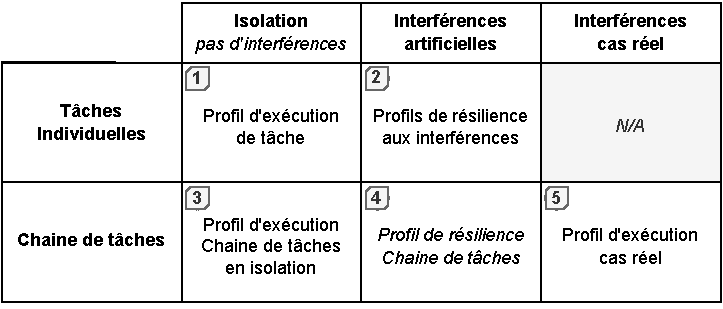
\includegraphics[width=0.7\linewidth]{Table_Protocole_Design}
        \end{table}
             
        Pour arriver à cet objectif, nous allons travailler sur deux paramètres dans le cadre de ce protocole expérimental. D'une part nous allons faire varier la charge utile, qui est le logiciel monitoré pour en tirer ses caractéristiques, et d'autre part nous modifions les interférences -- le stress -- subit par la charge utile. Les différentes étapes du protocole sont agrégées dans le Tableau~\ref{tab:tableprotocoledesign}. La charge utile sera au choix soit une tâche spécifique, soit une chaîne de tâches telle que définie dans le chapitre précédent, tandis qu'elle sera soumise soit \begin{enumerate*}[label=\bfseries\alph*)] \item à aucune interférence, donc isolation, soit \item avec des interférences "artificielles" par le biais de logiciels dédiés pour stresser au maximum le système, ou bien \item avec un cas "réel" d'interférences, constitué des tâches restantes du système qui auront été sélectionnées pour le cas d'étude.\end{enumerate*}
        Suivant ces composantes, le protocole de caractérisation se compose de cinq étapes, d'abord en caractérisant les tâches de façon individuelles, et ensuite en caractérisant les tâches critiques et la pertinence des choix de tâches au regard de l'ordonnançabilité et de la présence d'interférences logicielles : 
        \begin{itemize}
        	\item Profil d'exécution de chaque tâche
	        \begin{enumerate}[label=\large\ctxt{\arabic*}]
	        	\item tâches individuelles exécutées en isolation
	        	\item tâches individuelles exécutées avec le plus de stress possible
	        \end{enumerate}
        	\item Profil d'exécution de la chaîne de tâches critiques
        	\begin{enumerate}[resume*]
        		\item chaîne de tâche en condition d'exécution du mode dégradé 
        		\item chaîne de tâche exécutée avec le stress artificiel
        	\end{enumerate}
        	\item Set de tâche complet
        	\begin{enumerate}[resume*]
        		\item chaîne de tâche \& tâches non-critiques qui constituent le cas de test 
        	\end{enumerate}
        \end{itemize}
    

\subsection{Profil des tâches}
		Cette phase est nécessaire de façon à déterminer le profil d'exécution des tâches qui sont à notre disposition pour former un cas de test. Bien entendu, dans l'éventualité où l'on disposerait d'ores et déjà d'un jeu de tâches accompagné de leurs spécifications, tout cela n'est pas nécessaire et il conviendra uniquement de passer à l'étape~\ctxt{5} pour identifier la chaîne de tâche critique au regard du système et vérifier la pertinence d'implémenter un mécanisme de surveillance et contrôle selon les variations de temps de réponse sur les tâches critiques.
		
		L'objectif de la phase de profilage est d'avoir les connaissances suffisantes sur les tâches en termes de temps d'exécution à la fois en cas optimal (aucune interférence) et au cas où la tâche subit un stress sur l'utilisation de ressources partagées. À cet effet, on peut mesurer des éléments subsidiaires tels que l'espace mémoire occupé, le nombre d'appels systèmes et le profil de lecture/calcul/écriture des tâches pour une analyse plus fine. À l'issu de ces tests, on doit être capable de spécifier quelles seront les tâches sélectionnées pour constituer le cas de test, et parmi celles-ci, lesquelles serviront pour constituer la chaîne de tâche critique. Cette phase inclut donc les étapes \ctxt{1} et \ctxt{2}.
		
		\paragraph{\ctxt{1} - Tâches en Isolation}
			
			Cette première phase du processus consiste à exécuter une tâche individuelle sur la plateforme d'intégration en lui fournissant des données d'entrée de façon périodique. Sont mesurées les informations susmentionnées pour un nombre représentatif d'exécutions au regard de la variété possible des données d'entrée. 
			Ne connaissant pas l'ordre de grandeur des temps d'exécutions, il faudra prendre dans un premier temps une période d'exécution arbitraire (toutes les secondes par exemple). Il est possible ensuite de réduire ce temps pour que les tests soient plus rapides (toutes les 50ms pour une tâche qui prend autours de 20ms typiquement).
			
			Ces mesures expérimentales doivent être reproduites pour chaque tâche, de façon à obtenir une table des caractéristiques de chaque tâche en isolation.
                    
    	\paragraph{\ctxt{2} - Tâches avec stress imposé}
    		
    		De la même façon que pour l'étape précédente, l'objectif est d'obtenir les mêmes informations de profilage des tâches dans une mise en situation où le matériel est soumis à un niveau de stress élevé sur l'utilisation des caches, des entrées/sorties et en usage CPU, tandis que la tâche testée est exécutée périodiquement pour une durée suffisante de façon à obtenir un échantillon représentatif. Cela est dépendant du système et de la tâche en question.
    		
    		Les étapes avec un stress imposé sur le matériel nécessitent un logiciel dédié de stress. Plusieurs solutions sont possibles selon la plateforme de développement impliquée (matériel et logiciel). Pour mentionner quelques exemples, dans le cadre des travaux de~\cite{blin_maximizing_2016} des tâches dédiées ont été codées en assembleur pour effectuer des cycles d'accès mémoire sur une plateforme multicœur SABRE Lite. Sur des systèmes basés sur UNIX, il existe des outils comme \texttt{stress-ng}~\cite{king_stress-ng_2019} qui offrent toute une librairie d'utilitaires pour stresser des éléments spécifiques du processeur. 
    		
    		
	    	À l'issue de ces deux étapes de caractérisation, on dispose d'une matrice des caractéristiques du jeu de tâches qui inclut, pour chaque tâche tél qu'illustré dans le tableau: les temps d'exécutions minimum, médian, moyen et maximum, le nombre d'appels système, et éventuellement d'autres métriques propres à l'environnement d'exécution si elles sont pertinentes (nombre d'appels à un composant spécifique du firmware par exemple). À partir de ces données, on peut alors identifier~:
	    	\begin{enumerate}
	    		\item Les tâches qui ne sont pas adaptées à nos besoins pour un cas de test. Soit parce que l'ordre de grandeur des temps d'exécution n'est pas à la bonne échelle. Par exemple des tâches trop macroscopiques qui prennent plusieurs secondes de calcul alors que le reste du système de tâche est composé de micro-tâches monofonctionnelles qui s'exécutent en millisecondes. Soit parce qu'elles ont été codées d'une manière qui ne semble pas acceptable, par exemple avec une surutilisation des appels systèmes, qui provoquent des ralentissements indésirables trop dépendants du système d'exploitation.
	    		\item Les tâches qui sont appropriées pour servir de tâches non critiques qui vont provoquer des interférences. Ces dernières peuvent avoir des variations de temps d'exécution non négligeables, et utiliser des ressources partagées.
	    		\item Enfin, les tâches qui peuvent servir en tant que tâches critiques, qui représentent alors a minima des tâches temps-réel souple avec peu, voire pas d'appels système et un fonctionnement maîtrisé en isolation (variations de temps d'exécution raisonnables), et potentiellement sensibles à des interférences, donc avec une variation non négligeable du temps d'exécution médian entre les 2 conditions de test.   		
	    	\end{enumerate}
	    	
	    	\begin{table}
	    		\centering
				\caption{Table de caractérisation temporelle des tâches}
				\label{tab:tasksCaracs}
	    	\begin{tabular}{@{}c ccc c ccc cc@{}}
	    		\toprule
    			\mr{2}{Tâche}& \mr{2}{Appels Sys.} & \mr{2}{Autres appels} & \mc{3}{c}{en isolation} & \phantom{} & \mc{3}{c}{stressé} \\
	    		\cmidrule{4-6} \cmidrule{8-10}
	    		 & & & $ t_{min} $ & $ t_{max} $ & $ t_{med} $ &\phantom{} &  $ t_{min} $ & $ t_{max} $ & $ t_{med} $  \\
	    		\midrule
	    		$\tau_1$ & -- & -- & -- & -- & -- &  & -- & -- & -- \\
	    		... 	 & -- & -- & -- & -- & -- &  & -- & -- & -- \\
	    		$\tau_n$ & -- & -- & -- & -- & -- &  & -- & -- & -- \\
	    		\bottomrule
	    	\end{tabular}
   	    	\end{table} 		
    		
    		À l'issu de cette sélection, on a donc à disposition notre jeu de tâches, qui va être constitué d'une liste de tâches non critiques avec une période d'exécution pour chacune d'entre elle, et une liste de tâches critiques qui constituent la chaîne de tâches, qui doit donc inclure toutes les données relatives à la chaîne de tâche : fréquence d'exécution de chaque tâche, contraintes de précédence et échéance de temps de réponse bout-en-bout. 
    		Il s'avère que cette dernière donnée va être hautement dépendante des spécifications système, chose dont nous ne disposons pas ici. Par conséquent, il va falloir là encore proposer une façon de fixer cette contrainte, ou au moins en définir un ordre de grandeur qui pourra être ajusté selon la difficulté que l'on souhaite imposer au test. Plus cette échéance étant courte, plus il sera difficile de la garantir au regard des pires temps d'exécution des tâches. 
    		
                    
    \subsection{Profil du cas de test et Chaine de tâches}
    
L'objectif de cette seconde phase de caractérisation consiste justement à spécifier les tâches sélectionnées à plus haut niveau, notamment par la vérification de l'ordonnançabilité et de la contrainte de temps de réponse bout-en-bout de la chaîne.
		\paragraph{\ctxt{3} - Chaîne de tâches critique en isolation}
		Il est important de tester l'exécution de la chaîne de tâches en isolation, c'est-à-dire sans aucune interférence provenant des autres tâches qui doivent être intégrées. Cette étape permet de vérifier l'absence d'effets de bord entre la situation où les tâches étaient testées individuellement, et le cas qu'on l'on va viser comme étant le mode de fonctionnement dégradé pour garantir le temps de réponse désiré de la chaîne. En exécutant directement les tâches critiques dans ce mode dégradé, on peut donc d'une part connaître le profil de temps de réponse de la chaîne de tâche~: temps de réponse moyen, pire temps de réponse. À partir de cette information il devient possible de fixer dans notre spécification l'échéance de temps de réponse maximale permise pour la chaîne. Plus cette échéance sera proche du temps de réponse en mode dégradé, plus cela implique que cette échéance est stricte dans le sens où elle est plus courte et donc difficile à tenir en cas de perturbations. 
		Dans le cadre de nos expérimentations, nous fixons à cette étape deux éléments pour avancer dans les tests. Le premier sur la cohérence de la chaîne de tâche. Les tâches impliquées ici ayant un certain niveau de criticité, il semble pertinent de partir du principe qu'en l'absence de perturbations significatives l'écart entre le temps d'exécution minimal et maximal constatés pour la chaîne de tâche doivent être relativement restreints. Par conséquent, il faudra réviser le choix des tâches sélectionnées pour la chaîne dans le cas où l'on observe un écart trop significatif entre $ WCRT_{max} $ et $ WCRT_{min} $. Typiquement, si cet écart est supérieur la moitié du temps de réponse médian observé. Ce qu'on l'on peut formaliser comme~: si $ WCRT_{max} - WCRT_{min} \leq 0.5*WCRT_{median} $ en isolation, alors la chaîne est suffisamment cohérente dans son comportement nominal. 
		Si cette conclusion est remplie, alors le second élément sera l'échéance de temps de réponse de référence que l'on pourra se fixer comme spécification, qui sera $D_C = 2*WCRT_{median}$. Cela implique d'abord qu'en isolation, par définition on est garanti que la chaîne de tâche est ordonnançable et ne peut pas dépasser son échéance et ensuite que l'on pourra ajuster cette échéance pour tester l'efficacité du mécanisme de Surveillance et Contrôle, en ayant cette valeur de référence comme base pour tester une spécification plus ou moins contraignante et donc difficile à respecter en cas d'interférences.

		\paragraph{\ctxt{4} - Chaîne de tâches sous stress forcé}
		Il est possible de tirer parti des tâches de stress qui ont pu être utilisées pour la caractérisation individuelle de l'étape \ctxt{2} pour caractériser de la même façon la chaîne de tâche critique qui a été sélectionnée. L'objectif est de s'assurer de la pertinence d'implémenter le mécanisme de Surveillance et Contrôle dans le cas d'étude que nous sommes en train de construire, en vérifiant que la chaîne de tâche peut effectivement être sujette à des interférences qui mènent à un dépassement d'échéance. 
		Le test consiste logiquement à exécuter la chaîne de tâches critiques sélectionnée avec les paramètres de l'étape précédente, conjointement aux tâches dédiées à la mise en stress du processeur sur les ressources partagées. En toute logique, on doit constater des dépassements de l'échéance de manière significative. Si aucune variation n'est constatée comparé au cas où la chaîne est isolée, alors les tâches sélectionnées ne sont pas sujettes aux interférences et donc il ne sera pas utile d'y adjoindre de mécanisme de contrôle. La chaîne choisie n'est a priori pas pertinente pour un cas de test.

		\paragraph{\ctxt{5} - Système complet dont chaîne de tâche}
		Dans le cadre de mise en application de systèmes temps-réels à criticité mixte, il est nécessaire de passer par une phase de vérification d'ordonnançabilité. Cette phase est déjà partie intégrante des processus de développement industriels et propose de nombreux outils d'analyse tels que cela a été décrit dans le~\autoref{chap:2_StateofArt}. Nous n'avons pas approfondi en détail cette dimension de l'implémentation d'un set de tâches pour nous focaliser sur la proposition d'un mécanisme en lui-même en supposant que les vérifications d'usage d'ordonnançabilité sont validées. Il faut notamment noter que notre démarche véhicule l'espoir d'alléger les contraintes de garanties d'ordonnançabilité dans une certaine mesure. Notre positionnement étant que par la possibilité de passer dans un mode dégradé qui permet de façon transitoire la garantie d'ordonnançabilité d'un sous-ensemble des tâches alors les preuves d'ordonnançabilité par estimation de pire temps d'exécution peuvent être allégées sur les tâches ciblées par le mécanisme.
		
		Par conséquent, dans cette étape, nous réalisons les vérifications sur l'ordonnançabilité du jeu de tâches sélectionnées sans chercher un niveau de vérification strict. De fait, sachant que l'on peut se permettre des dépassements d'échéances de façon marginale sur les tâches non-critiques (par définition) et sur les tâches critiques (avec la perspective de compenser cela via le mécanisme). Cette vérification est faite expérimentalement en reprenant les jeux de tests des étapes précédentes, mais cette fois-ci avec toutes les tâches exécutées aux périodes d'exécutions fixées empiriquement. L'ordonnançabilité est donc testée en premier lieu de façon grossière via le calcul de taux d'occupation CPU moyen qui peut être ajusté avec la période d'exécution des tâches suivant la formule~:	$ \sum{\dfrac{C_i}{T_i}} \leq 1 $ pour toutes les tâches allouées au même cœur pour un ordonnancement partitionné, ou \alert{ajouter ici calcul taux utilisation du CPU} $  $ pour un ordonnancement global (c.-à-d. sans d'allocation des tâches).
			
		Dans un second temps la vérification est faite expérimentalement en surveillant l'exécution correcte des tâches selon les périodes fixées dans une mise en situation réelle la plus représentative possible.
		 
		\comment{Choix du temps d'expérimentation et jeu de données d'entrée}{J'ai un peu éludé sur la question de combien de temps doivent durer les expérimentations et sur les éventuelles données d'entrée à utiliser qui se doivent représentatives et espérer couvrir les pires cas... C'est un "gros" morceaux en termes de temps que ça aurait demandé pour être fait de façon totalement exhaustive (la thèse de Mohammed est totalement dédiée à ça si je ne m'abuse) donc j'ai peur qu'en mettant le doigt dedans je complique trop les choses sans y apporter de réponse satisfaisante.}
		
		Cette étape permet aussi d'ores-et-déjà de constater le comportement de la chaîne de tâche dans le cas nominal en l'absence de mécanisme pour contrôler d'éventuels augmentations indésirables de son temps de réponse. Il faut comparer ces temps de réponse avec les résultats obtenus à l'étape \ctxt{3}, qui correspond au mode dégradé où la chaîne est en isolation. Cela permet de quantifier l'influence spécifique à notre cas d'étude des interférences sur les tâches critiques et d'étudier la pertinence du choix d'échéance bout-en-bout qui a été fait à cette même étape. De fait, selon les temps de réponse constatés en fonctionnement normal sans mécanisme, sachant que la vérification de l'influence d'interférences a été effectuée à l'étape précédente, il est alors possible de voir si les tâches non-critique choisies ont effectivement, elles aussi, un effet significatif sur l'usage des ressources partagées. Si la chaîne de tâche conserve un profil d'exécution similaire au mode dégradé, on est en mesure de dire que les tâches non-critiques choisies ne sont pas suffisantes pour avoir une influence sur les ressources partagées.
		
		Après avoir validé la définition des tâches critiques à l'étape précédente, on valide donc ici la définition des tâches non-critiques et donc du cas de test dans son ensemble.
		
		
		%%Expected result is a schedulable system with reference task chain response times with interferences.
                	

                	
                	
\section{Phase de Calibration}

            \begin{table}[ht]
				\centering
				\caption{Protocole d'implémentation et calibration du mécanisme}
				\label{tab:tableprotocoleImplementation}
				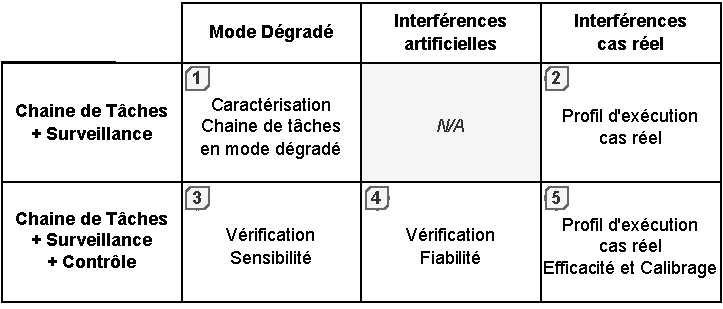
\includegraphics[width=0.7\linewidth]{Table_Protocole_Implem}
			\end{table}
            This phase is mandatory to configure the Control mechanism to the software and hardware specificities and lower false-positive rate. It is made of steps \ctxt{4}, \ctxt{5}, \ctxt{6} in orange boxes of \autoref{tab:tableprotocoledesign}. Configuration includes task chain worst-case response time and intermediary response times in isolation. Performance optimisation consist in tweaking the switch time $t_{sw}$ and anticipation execution frequency $W_{max}$ constants, in the objective of lowering false-positive anticipation rates.
            
    \subsection{Chaine de tâches avec stress forcé}
                    The task chain is then tested under a worst-case scenario. It is executed with the artificial system load, to stress as much as possible the task chain similarly to step \ctxt{2}. We get a baseline of the worst-case chain response time. This value is important because if the end-to-end deadline is always greater than the worst-case response time observed then the mechanism would be of no use (i.e. deadline never broken from temporal faults). This step gives a quantification of the task chain sensitivity to interferences and thus indicates the pertinence of using a Monitoring and Control Agent to manage them.
                    
    \subsection{Chaine de tâche en isolation}
                    The objective is to calibrate Control mechanism parameters~: $rWCRT(\tau_i)$, Core Control Component period ($T_{CCC}$) and switch time ($t_{sw}$) to degraded mode. The task chain is executed alone with the MCA but with the Control mode switch disabled. We log every chain intermediary and end-to-end response times. The result gives the data of all the remaining response times obtained during the test. We set the $rWCRT(\tau_i)$ parameters as an upper limits of the remaining response times registered.
                    
    \subsection{Chaine de tâche avec mécanisme de Contrôle}
                	Finally, the Control mechanism is enabled, with the parameters set on previous step. As this step does not include the LO tasks that bring interferences to the task chain, the Core Control Component should not trigger any switch to degraded mode. This step is important for the final analysis as it already points out the base false positive rate obtained with chosen parameters. A qualitative MCA should have the least degraded mode switch possible. Otherwise it could mean that either the CCC parameters are not ideally set (typically $W_{max}$), or the expected timing delays caused from interferences are too close to the usual timing variation of the task chain execution even in isolation. In other words, the Control Component is not able to differentiate response time variations due to temporal faults from ones due to nominal execution time variations. Another possibility is the end-to-end deadline requirement is too close to the nominal end-to-end response time in isolation. %If this has no effect then it could just mean that regarding step \ctxt{4}, the task chain is not subject to timing faults.
                	
                	
\section{Phase de Validation en exécution}
    \subsection{Chaine de tâches avec système complet et mécanisme de Contrôle}
                    The validation phase implies a last step (\ctxt{7} in green box of \autoref{tab:tableprotocoleImplementation}), which is with the whole final system being executed~: HI task chain and LO tasks with the MCA enabled. The objective is to collect the concluding information on the Monitoring and Control Agent behavior to measure the 3 quantification criteria (efficiency, performance and quality) of the solution explained in \autoref{eq:safe_cond}. We also use the data from steps \ctxt{3} and \ctxt{6} as a reference for the conclusions.
\ifdefined\included
\else
\bibliographystyle{StyleThese}
\bibliography{these}
\end{document}
\fi
